%------------------------------------------------------------------------------
% Author(s):
% Varaun Ramgoolie
%
% Copyright:
%  Copyright (C) 2020 Brad Bachu, Arjun Mohammed, Varaun Ramgoolie, Nicholas Sammy
%
%  This file is part of Applied-Mathematics-Unit2 and is distributed under the
%  terms of the MIT License. See the LICENSE file for details.
%
%  Description:
%     Year: 2005 C
%     Module: 3
%     Question: 6 Sketch 1
%------------------------------------------------------------------------------

\documentclass[crop,tikz]{standalone}
\usetikzlibrary{scopes,calc,patterns,angles,quotes}

\begin{document}
	
	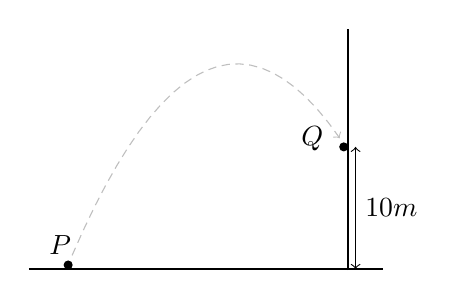
\begin{tikzpicture}
		

			%\draw[step = 0.5cm, very thin, gray] (0,0) grid (5,5);
			
			
			%draw floor and wall
			\draw [thick] (0,0.45) -- (4.5,0.45);
			\draw [thick] (4.05,0.435) -- (4.05,3.5);
			
			%two circles as point particles	
			\draw [draw=black,fill=black] (0.5,0.5) circle [radius=0.05];
			\draw [draw=black,fill=black] (4,2) circle [radius=0.05];
			
			
			
			% path
			\draw  [->, domain=0.55:3.95, densely dashed,gray!50,font=\small] plot (\x, {-0.55451 *\x*\x +  2.93287*\x - 0.823308});
			
			
			%naming points P and Q
			\draw[] (0.4,0.75) node{$P$};
			\draw[] (3.6,2.1) node{$Q$};
			
			
			%measurement
			\draw[<->] (4.15,0.45)--(4.15,2) node[midway,right]{$10m$};

			
			%&
			%\draw[step = 0.5cm, very thin, gray] (0,0) grid (4,4);
			%\draw[->, thick] (0,0.5)--(0,1.5) node[left]{$+y$};
			%\draw[->, thick] (0,0.5)--(1,0.5) node[right]{$+x$};
			\\		
		
		
		
	\end{tikzpicture}
	
\end{document}